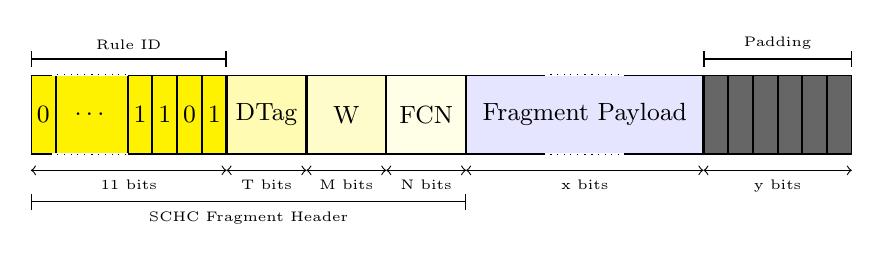
\begin{tikzpicture}

\draw (0,0) node (b1)  [rectangle, draw, minimum height=1cm, minimum width = 0.3cm, fill=yellow] {};
\draw(b1) node {\small{0}};
\draw (b1.east) node (b2)  [right, rectangle, draw, minimum height=1cm, minimum width = 0.9cm, fill=yellow] {};
\draw(b2) node {\small{\dots}};


\draw [white, thick] (b2.north) -- +(0.5, 0);
\draw [white, thick] (b2.north) -- +(-0.5, 0);

\draw [dotted] (b2.north) -- +(0.5, 0);
\draw [dotted] (b2.north) -- +(-0.5, 0);

\draw [white, thick] (b2.south) -- +(0.5, 0);
\draw [white, thick] (b2.south) -- +(-0.5, 0);

\draw [dotted] (b2.south) -- +(0.5, 0);
\draw [dotted] (b2.south) -- +(-0.5, 0);


\draw (b2.east) node (b8)  [right, rectangle, draw, minimum height=1cm, minimum width = 0.3cm, fill=yellow] {};
\draw(b8) node {\small{1}};

\draw (b8.east) node (b9)  [right, rectangle, draw, minimum height=1cm, minimum width = 0.3cm, fill=yellow] {};
\draw(b9) node {\small{1}};

\draw (b9.east) node (b10)  [right, rectangle, draw, minimum height=1cm, minimum width = 0.3cm, fill=yellow] {};
\draw(b10) node {\small{0}};

\draw (b10.east) node (b11)  [right, rectangle, draw, minimum height=1cm, minimum width = 0.3cm, fill=yellow] {};
\draw(b11) node {\small{1}};
\path(b1.north) -- +(0, 0.2) coordinate(hlineu);

\draw [|-|] (b1.west |- hlineu) -- coordinate(a) (b11.east |- hlineu) ;
\draw (a) node [above] {\tiny{Rule ID}};
\path(b1.south) -- +(0, -0.2) coordinate(hline);

\draw [<->] (b1.west |- hline) -- coordinate(a) (b11.east |- hline) ;
\draw (a) node [below] {\tiny{11 bits}};
\draw (b11.east) node (dtag) [right, rectangle, draw, minimum height=1cm, minimum width=1cm, fill=yellow!30]{};
\draw (dtag) node {\small{DTag}};
\path(b1.south) -- +(0, -0.2) coordinate(hline);


\path(b1.south) -- +(0, -0.2) coordinate(hline);
\draw [<->] (dtag.west |- hline) -- coordinate(a) (dtag.east |- hline) ;
\draw (a) node [below] {\tiny{T bits}};


\draw (dtag.east) node (w) [right, rectangle, draw, minimum height=1.0cm, minimum width=1cm, fill=yellow!20]{};
\draw (w) node {\small{W}};

\draw [<->] (w.west |- hline) -- coordinate(a) (w.east |- hline) ;
\draw (a) node [below] {\tiny{M bits}};


\draw (w.east) node (fcn) [right, rectangle, draw, minimum height=1cm, minimum width=1cm, fill=yellow!10]{};
\draw (fcn.text) node {\small{FCN}};

\draw [<->] (fcn.west |- hline) -- coordinate(a) (fcn.east |- hline) ;
\draw (a) node [below] {\tiny{N bits}};

\draw (fcn.east) node (fpay) [right, rectangle, draw, minimum height=1cm, minimum width=3cm, fill=blue!10]{};
\draw (fpay.text) node {\small{Fragment Payload}};

\draw [white, thick] (fpay.north) -- +(0.5, 0);
\draw [white, thick] (fpay.north) -- +(-0.5, 0);
\draw [dotted] (fpay.north) -- +(0.5, 0);
\draw [dotted] (fpay.north) -- +(-0.5, 0);

\draw [white, thick] (fpay.south) -- +(0.5, 0);
\draw [white, thick] (fpay.south) -- +(-0.5, 0);
\draw [dotted] (fpay.south) -- +(0.5, 0);
\draw [dotted] (fpay.south) -- +(-0.5, 0);

\draw [<->] (fpay.west |- hline) -- coordinate(a) (fpay.east |- hline) ;
\draw (a) node [below] {\tiny{x bits}};

\draw (fpay.east) node (p1)  [right, rectangle, draw, minimum height=1cm, minimum width = 0.3cm, fill=black!60] {};
\draw (p1.east) node (p2)  [right, rectangle, draw, minimum height=1cm, minimum width = 0.3cm, fill=black!60] {};
\draw (p2.east) node (p3)  [right,rectangle, draw, minimum height=1cm, minimum width = 0.3cm, fill=black!60] {};
\draw (p3.east) node (p4)  [right,rectangle, draw, minimum height=1cm, minimum width = 0.3cm, fill=black!60] {};
\draw (p4.east) node (p5)  [right,rectangle, draw, minimum height=1cm, minimum width = 0.3cm, fill=black!60] {};
\draw (p5.east) node (p6)  [right,rectangle, draw, minimum height=1cm, minimum width = 0.3cm, fill=black!60] {};

\path(b1.south) -- +(0, - 0.6) coordinate(hline1);
\draw [|-|] (b1.west |- hline1) -- coordinate(a) (fcn.east |- hline1) ;
coordinate 
\draw (a) node [below] {\tiny{SCHC Fragment Header}};


\draw [|-|] (p1.west |- hlineu) -- coordinate(a) (p6.east |- hlineu) ;
\draw (a) node [above] {\tiny{Padding}};

\draw [<->] (p1.west |- hline) -- coordinate(a) (p6.east |- hline) ;
\draw (a) node [below] {\tiny{y bits}};

\end{tikzpicture}
